\documentclass{article}

\usepackage[margin = 1in]{geometry}
\usepackage{booktabs}
\usepackage{graphicx}
\usepackage{epstopdf}


\begin{document}

\title{10-601 Machine Learning - Homework 4 Report}
\author{Dawei Wang \\ {\tt daweiwan@andrew.cmu.edu}}

\maketitle

\begin{table}[h!]
	\centering
	\caption{95\% and 99\% Confidence Interval for $k=2$ and $k=10$}\vspace{4pt}
	\label{confinterval}
	\begin{tabular}{cccccc} \toprule
	\multicolumn{3}{c}{$k=2$} & \multicolumn{3}{c}{$k=10$} \\ \midrule
	Acc & .95\% & .99\% &	Acc & .95\% & .99\% \\ \midrule
	64.0\% & [0.546, 0.734] & [0.516, 0.764] & 70.0\% & [0.499, 0.901] & [0.436, 0.964] \\ 
	73.0\% & [0.643, 0.817] & [0.616, 0.844] & 80.0\% & [0.625, 0.975] & [0.570, 1.030] \\
	70.0\% & [0.610, 0.790] & [0.582, 0.818] & 55.0\% & [0.332, 0.768] & [0.263, 0.837] \\
	70.0\% & [0.610, 0.790] & [0.582, 0.818] & 65.0\% & [0.441, 0.859] & [0.375, 0.925] \\
	68.0\% & [0.589, 0.771] & [0.560, 0.800] & 55.0\% & [0.332, 0.768] & [0.263, 0.837] \\
	64.0\% & [0.546, 0.734] & [0.516, 0.764] & 65.0\% & [0.441, 0.859] & [0.375, 0.925] \\
	70.0\% & [0.610, 0.790] & [0.582, 0.818] & 80.0\% & [0.625, 0.975] & [0.570, 1.030] \\
	73.0\% & [0.643, 0.817] & [0.616, 0.844] & 70.0\% & [0.499, 0.901] & [0.436, 0.964] \\
	78.0\% & [0.699, 0.861] & [0.673, 0.887] & 80.0\% & [0.625, 0.975] & [0.570, 1.030] \\
	76.0\% & [0.676, 0.844] & [0.650, 0.870] & 65.0\% & [0.441, 0.859] & [0.375, 0.925] \\ \bottomrule
	\end{tabular}
\end{table}

\noindent {\bf Held-out Set Test} The test was carried out for ten times.
See Table \ref{confinterval} for the result. \\
{\bf Observation} Larger $k$ results in wider confidence intervals and more fluctating accuracies. 

\begin{figure}[h!]
	\centering
	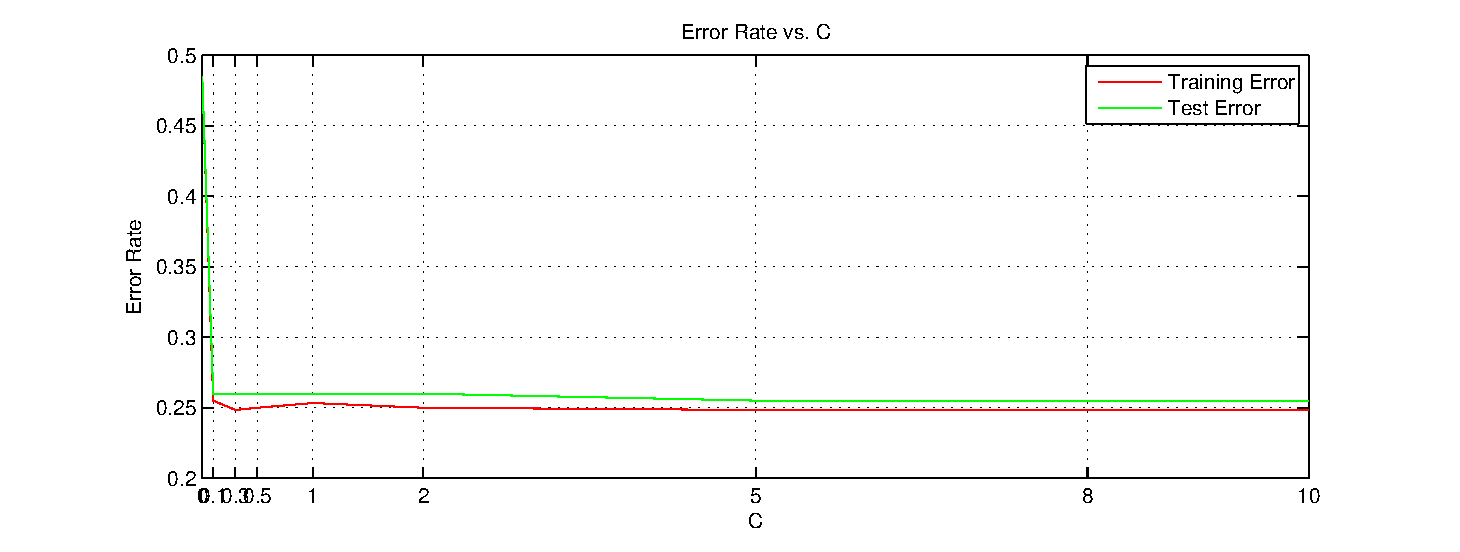
\includegraphics[width=0.8\paperwidth]{ploterr.eps}
	\caption{Error Rate versus $C$}\label{errorrate-c}
\end{figure}

\noindent {\bf Find C by Cross-Validation} The test was carried out for five times. 
See Figure \ref{errorrate-c} for the result. The red polylines correspond to the training errors, 
and the green to the testing errors. \\
{\bf Observation} $C=0.1$ yields the best training and testing errors for this particular set of data.

\begin{table}
	\centering
	\caption{LR and NN Comparison: Error Rate}\vspace{4pt}\label{lr-nn}
	\begin{tabular}{ccccccccccc} \toprule
	   AL & 1 & 2 & 3 & 4 & 5 & 6 & 7 & 8 & 9 & 10 \\ \midrule
	   LR & 0.000 & 0.000 & 0.000 & 0.091 & 0.000 & 0.000 & 0.045 & 0.000 & 0.000 & 0.000 \\
	   NN & 0.000 & 0.000 & 0.000 & 0.091 & 0.000 & 0.000 & 0.045 & 0.000 & 0.000 & 0.000 \\ \midrule
	   LR & 0.045 & 0.000 & 0.000 & 0.000 & 0.000 & 0.000 & 0.091 & 0.000 & 0.000 & 0.000 \\
	   NN & 0.045 & 0.000 & 0.000 & 0.000 & 0.000 & 0.000 & 0.091 & 0.000 & 0.000 & 0.000 \\ \midrule
	   LR & 0.000 & 0.045 & 0.045 & 0.000 & 0.000 & 0.000 & 0.000 & 0.045 & 0.000 & 0.000 \\
	   NN & 0.000 & 0.045 & 0.045 & 0.000 & 0.000 & 0.000 & 0.000 & 0.045 & 0.000 & 0.000 \\ \midrule
	   LR & 0.045 & 0.000 & 0.000 & 0.045 & 0.000 & 0.000 & 0.045 & 0.045 & 0.000 & 0.000 \\
	   NN & 0.000 & 0.000 & 0.000 & 0.045 & 0.000 & 0.000 & 0.045 & 0.045 & 0.000 & 0.000 \\ \midrule
	   LR & 0.000 & 0.000 & 0.000 & 0.000 & 0.000 & 0.000 & 0.000 & 0.000 & 0.045 & 0.087 \\
	   NN & 0.000 & 0.000 & 0.000 & 0.000 & 0.000 & 0.000 & 0.000 & 0.000 & 0.045 & 0.087 \\ \bottomrule
	\end{tabular}
\end{table}

\vspace{2cm}
\noindent {\bf LR and NN Comparison} Only the instances labeled with 4 and 7 are used in this test.
Both classifiers were first trained on the filtered {\tt Xtrain} and {\tt Ytrain}, then tested against 
10 disjoint subsets obtained by partitioning the filtered {\tt Xtest} and {\tt Ytest}. See Table \ref{lr-nn} for the result. Only the fourth group shows difference. 
{\bf Observation} For the group that shows difference: $p=0.343$ under two-tailed test, $p=0.171$ under one-tailed test;
but it's not significant enough to assert which one is better. For this particular data-set, they 
have performed equally well. 



\end{document}











